%% LaTeX poster using beamerposter
\documentclass[final]{beamer}

%% Load beamerposter package
\usepackage[size=a0,scale=1.0]{beamerposter}

%% Set theme and colors
\usetheme{ConfPoster}
\usecolortheme{default}
\usepackage{graphicx, booktabs, multicol}
\usepackage{lipsum} %% for placeholder text

%% Poster title and authors
\title{EFI Theory: Quantifying Ecological Predictability and Advancing Ecological Theory via Forecasting}
\author{Cole Brookson, Abby Lewis, Shubhi Sharma, Caleb Robbins, Bilgecan \c{S}en}
\date{Ecological Forecasting Initiative Conference 2025}

%% Begin document
\begin{document}

\begin{frame}[t]

\begin{columns}[t,totalwidth=0.99\textwidth]

% Left column ------------------------------------------------------------------
\begin{column}{0.32\textwidth}
  \begin{block}{Introduction}
    The EFI Theory working group has been working for \~3 years to understand how ecological forecasting can improve our understanding of predictability across systems and scales. This work is structured around three aims relying on single data streams:
  \end{block}

  \begin{block}{Data Sources}
    We use NEON data streams including carbon cycling, water quality, beetle abundance, plant phenology, and tick dynamics, with weather drivers from NOAA.
  \end{block}

  \begin{block}{Aim 1: Forecast Performance}
    Theory group members have developed >10,000 probabilistic forecasts across 11 models. We analyze forecast skill (e.g., RMSE) as a function of forecast horizon using GAMs. Results suggest horizon has a nonlinear effect on skill.

    \vspace{1em}
    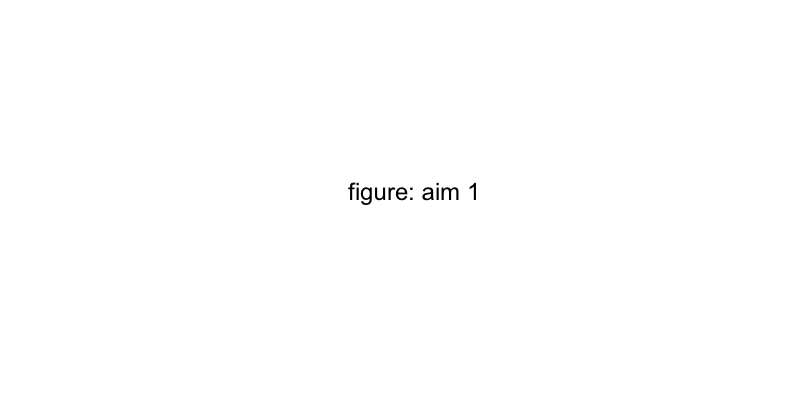
\includegraphics[width=0.95\linewidth,height=0.25\textheight]{figures/aim1-placeholder.png} % placeholder
  \end{block}
\end{column}

% Middle column ----------------------------------------------------------------
\begin{column}{0.32\textwidth}
  \begin{block}{Aim 2: Uncertainty and Predictability}
    We are evaluating how different sources of uncertainty (e.g., process vs parameter) influence predictability across ecological systems. Forecast skill is linked to uncertainty sources through decomposition methods.
  \end{block}

  \begin{block}{Aim 3: Theoretical Framework}
    Using entropy-based measures, we assess the limits of predictability and how close current forecasts come to those limits. We identify dominant sources of error and explore conceptual links across disciplines.

    \vspace{1em}
    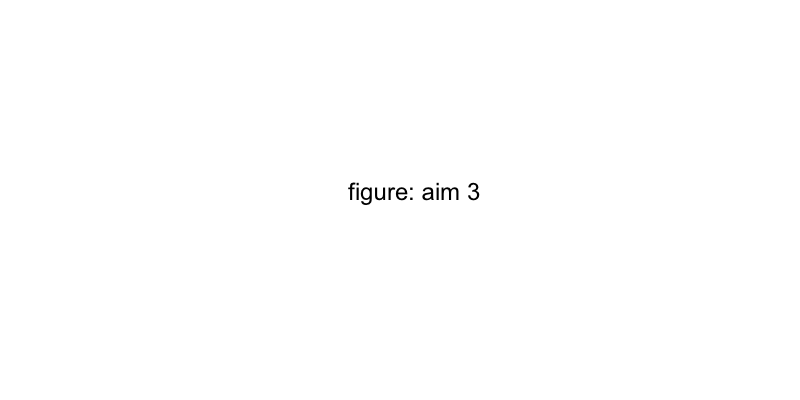
\includegraphics[width=0.95\linewidth,height=0.25\textheight]{figures/aim3-placeholder.png} % placeholder
  \end{block}
\end{column}

% Right column -----------------------------------------------------------------
\begin{column}{0.32\textwidth}
  \begin{exampleblock}{Conceptual Synthesis}
    At EFI2025, we outline a framework for how ecological forecasts contribute to an interdisciplinary understanding of predictability. We synthesize concepts from philosophy, statistics, and the natural sciences.
  \end{exampleblock}

  \begin{alertblock}{Want to get involved?}
    Scan this QR code to learn more about the Theory Working Group!
    
    \vspace{1em}
    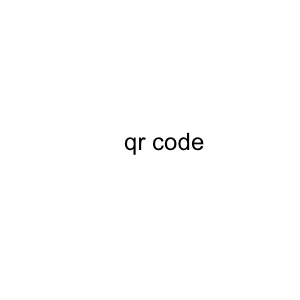
\includegraphics[width=0.6\linewidth]{figures/qr-placeholder.png} % placeholder
  \end{alertblock}
\end{column}

\end{columns}

\end{frame}

\end{document}
